% Figure 2: Two-layer determination model and cell-type analysis (TikZ)
\begin{figure}[!ht]
\centering

% ── Grayscale palette ──
\definecolor{cL1}{gray}{0.35}       % Layer 1: dark gray
\definecolor{cL1light}{gray}{0.92}  % Layer 1 background
\definecolor{cL1mid}{gray}{0.45}    % Layer 1 mid-tone
\definecolor{cL1dark}{gray}{0.20}   % Layer 1 darkest
\definecolor{cL2}{gray}{0.50}       % Layer 2: medium gray
\definecolor{cL2light}{gray}{0.92}  % Layer 2 background
\definecolor{cL2mid}{gray}{0.55}    % Layer 2 mid-tone
\definecolor{cL2dark}{gray}{0.30}   % Layer 2 darkest
\definecolor{cBoundary}{gray}{0.40}
\definecolor{cGrid}{gray}{0.88}
\definecolor{cText}{gray}{0.15}
\definecolor{cAnnot}{gray}{0.60}
\definecolor{cGapBorder}{gray}{0.65}
\definecolor{cGapFill}{gray}{0.95}
\definecolor{cGapText}{gray}{0.30}

% ═══════════════════════════════════════════════════════════════
% Panel (a): Cascade architecture (full width)
% ═══════════════════════════════════════════════════════════════
\textbf{(a)}\par\vspace{0.3em}
\begin{tikzpicture}[
    x=1cm, y=1cm,
    flowbox/.style={draw=#1!40!black, rounded corners=3pt, fill=#1,
                    minimum width=1.7cm, minimum height=0.65cm,
                    font=\scriptsize\bfseries, text=white,
                    line width=0.3pt, align=center},
    metricbadge/.style={rounded corners=2pt, fill=#1, opacity=0.85,
                        font=\tiny\bfseries, text=white,
                        inner sep=2.5pt},
    arr/.style={-{Stealth[length=1.5mm, width=1mm]}, #1, line width=0.6pt},
]

% ── Layer 1 background band ──
\fill[cL1light, rounded corners=4pt]
    (0, 2.5) rectangle (9.5, 5.0);
\draw[cL1, line width=0.5pt, rounded corners=4pt]
    (0, 2.5) rectangle (9.5, 5.0);
\node[font=\tiny\itshape, text=cL1, anchor=west] at (0.15, 4.8)
    {Layer 1: Sequence-determined};

% Layer 1 boxes
\node[flowbox=cL1]
    (protseq) at (1.2, 4.15) {Protein\\sequence};
\node[flowbox=cL1mid]
    (sitepos) at (1.2, 3.15) {Site\\position};
\node[flowbox=cL1]
    (esm2) at (3.6, 3.65) {ESM-2 +\\retrieval\\model};
\node[flowbox=cL1dark]
    (cluster) at (6.0, 3.65) {Cluster\\(K\,=\,20)};
\node[metricbadge=cL1] at (8.0, 3.65) {H@5 = 0.786};

% Layer 1 arrows
\draw[arr=cL1] (protseq.east) -- (esm2.170);
\draw[arr=cL1] (sitepos.east) -- (esm2.190);
\draw[arr=cL1] (esm2.east) -- (cluster.west);

% ── Layer 2 background band ──
\fill[cL2light, rounded corners=4pt]
    (0, 0.0) rectangle (9.5, 2.2);
\draw[cL2, line width=0.5pt, rounded corners=4pt]
    (0, 0.0) rectangle (9.5, 2.2);
\node[font=\tiny\itshape, text=cL2, anchor=west] at (0.15, 2.0)
    {Layer 2: Environment-determined};

% Layer 2 boxes
\node[flowbox=cL2]
    (celltype) at (1.2, 1.05) {Cell-type\\enzyme expr.};
\node[flowbox=cL2mid]
    (scoring) at (3.6, 1.05) {Enzyme\\scoring};
\node[flowbox=cL2dark]
    (glycanid) at (6.0, 1.05) {Glycan ID};
\node[metricbadge=cL2] at (8.0, 1.05) {MRR = 0.066};

% Layer 2 arrows
\draw[arr=cL2] (celltype.east) -- (scoring.west);
\draw[arr=cL2] (scoring.east)  -- (glycanid.west);

% ── Cross-boundary arrow (dashed) ──
\draw[-{Stealth[length=1.5mm, width=1mm]}, cBoundary,
      line width=0.7pt, dashed]
    (cluster.south) .. controls +(0,-0.5) and +(0.8,0.7) .. (scoring.north);

% ── Data-gap callout ──
\node[draw=cGapBorder, rounded corners=3pt,
      fill=cGapFill, line width=0.4pt,
      font=\tiny, text=cGapText, align=center]
    at (10.5, 1.05) {39\% glycans with\\enzyme annotations};

\end{tikzpicture}

\vspace{1.2em}

% ═══════════════════════════════════════════════════════════════
% Bottom row: (b) left, (c) right
% ═══════════════════════════════════════════════════════════════
\begin{minipage}[t]{0.47\textwidth}
\centering

% ═══════════════════════════════════════════════════════════════
% Panel (b): Two-layer conceptual model
% ═══════════════════════════════════════════════════════════════
\textbf{(b)}\par\vspace{0.3em}
\begin{tikzpicture}[x=0.95cm, y=1cm]

% ── Layer 1 band ──
\fill[cL1light, rounded corners=4pt] (1.2, 2.6) rectangle (7.0, 4.6);
\draw[cL1, line width=0.6pt, rounded corners=4pt] (1.2, 2.6) rectangle (7.0, 4.6);
\node[font=\scriptsize\bfseries, text=cL1] at (4.1, 4.2)
    {Layer 1: Sequence-determined};
\node[font=\tiny, text=cText, align=center] at (4.1, 3.4)
    {Site classification (F1 = 0.924)\\
     Type prediction (Acc = 0.844)\\
     Structural cluster (H@5 = 0.786)};

% ── Boundary dashed line ──
\draw[cBoundary, dashed, line width=0.7pt, opacity=0.7] (1.3, 2.35) -- (6.9, 2.35);

% ── Layer 2 band ──
\fill[cL2light, rounded corners=4pt] (1.2, 0.3) rectangle (7.0, 2.1);
\draw[cL2, line width=0.6pt, rounded corners=4pt] (1.2, 0.3) rectangle (7.0, 2.1);
\node[font=\scriptsize\bfseries, text=cL2] at (4.1, 1.7)
    {Layer 2: Environment-determined};
\node[font=\tiny, text=cText, align=center] at (4.1, 0.95)
    {Exact glycan ID (MRR = 0.066--0.118)\\
     Enzyme expr.\;\;|\;\;Golgi transit\;\;|\;\;NTP sugars};

% ── 10× gap annotation ──
\draw[{Stealth[length=1.5mm]}-{Stealth[length=1.5mm]}, cText, line width=0.8pt]
    (7.8, 1.2) -- (7.8, 3.6);
\node[font=\scriptsize\bfseries, text=cText, fill=white, inner sep=1pt]
    at (7.8, 2.4) {10$\times$\,gap};

% ── Side annotations ──
\node[font=\tiny\itshape, text=cL1, align=center, anchor=east] at (1.0, 3.6)
    {Predictable\\from sequence};
\node[font=\tiny\itshape, text=cL2, align=center, anchor=east] at (1.0, 1.2)
    {Requires\\cellular context};

\end{tikzpicture}
\end{minipage}%
\hfill%
\begin{minipage}[t]{0.50\textwidth}
\centering

% ═══════════════════════════════════════════════════════════════
% Panel (c): Performance across hierarchy — horizontal bars
% ═══════════════════════════════════════════════════════════════
\textbf{(c)}\par\vspace{0.3em}
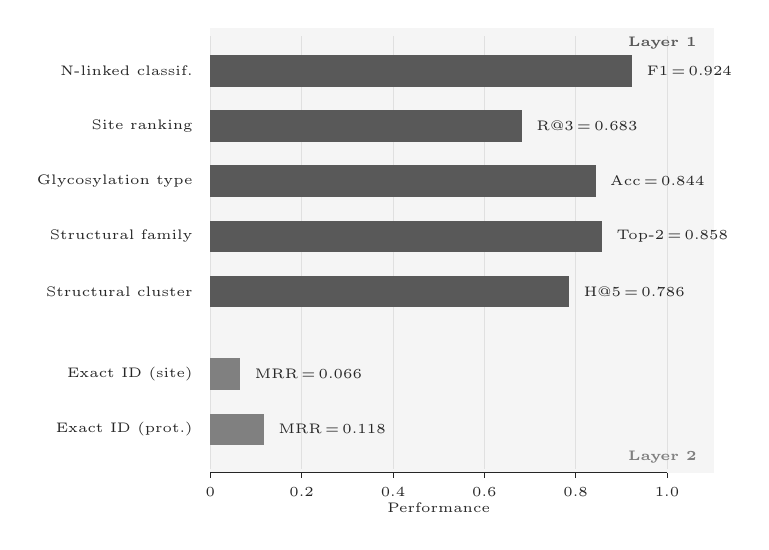
\begin{tikzpicture}[x=1cm, y=1cm]

\pgfmathsetmacro{\bs}{5.8}

% ── Layer background spans ──
\fill[cL1light, opacity=0.5] (0, 1.4) rectangle (\bs+0.6, 5.3);
\fill[cL2light, opacity=0.5] (0, -0.35) rectangle (\bs+0.6, 1.4);

% ── Grid lines ──
\foreach \gx in {0,0.2,...,1.0}
    \draw[cGrid, line width=0.2pt] (\gx*\bs, -0.3) -- (\gx*\bs, 5.2);

% ── Layer labels ──
\node[font=\tiny\bfseries, text=cL1, anchor=east] at (\bs+0.5, 5.1) {Layer 1};
\node[font=\tiny\bfseries, text=cL2, anchor=east] at (\bs+0.5, -0.15) {Layer 2};

% ── Bars (Layer 1: dark gray) ──
\fill[cL1] (0, 4.55) rectangle (0.924*\bs, 4.95);
\node[anchor=east, font=\tiny, text=cText] at (-0.1, 4.75) {N-linked classif.};
\node[anchor=west, font=\tiny, text=cText] at (0.924*\bs+0.06, 4.75) {F1\,=\,0.924};

\fill[cL1] (0, 3.85) rectangle (0.683*\bs, 4.25);
\node[anchor=east, font=\tiny, text=cText] at (-0.1, 4.05) {Site ranking};
\node[anchor=west, font=\tiny, text=cText] at (0.683*\bs+0.06, 4.05) {R@3\,=\,0.683};

\fill[cL1] (0, 3.15) rectangle (0.844*\bs, 3.55);
\node[anchor=east, font=\tiny, text=cText] at (-0.1, 3.35) {Glycosylation type};
\node[anchor=west, font=\tiny, text=cText] at (0.844*\bs+0.06, 3.35) {Acc\,=\,0.844};

\fill[cL1] (0, 2.45) rectangle (0.858*\bs, 2.85);
\node[anchor=east, font=\tiny, text=cText] at (-0.1, 2.65) {Structural family};
\node[anchor=west, font=\tiny, text=cText] at (0.858*\bs+0.06, 2.65) {Top-2\,=\,0.858};

\fill[cL1] (0, 1.75) rectangle (0.786*\bs, 2.15);
\node[anchor=east, font=\tiny, text=cText] at (-0.1, 1.95) {Structural cluster};
\node[anchor=west, font=\tiny, text=cText] at (0.786*\bs+0.06, 1.95) {H@5\,=\,0.786};

% ── Bars (Layer 2: medium gray) ──
\fill[cL2] (0, 0.7) rectangle (0.066*\bs, 1.1);
\node[anchor=east, font=\tiny, text=cText] at (-0.1, 0.9) {Exact ID (site)};
\node[anchor=west, font=\tiny, text=cText] at (0.066*\bs+0.06, 0.9) {MRR\,=\,0.066};

\fill[cL2] (0, 0.0) rectangle (0.118*\bs, 0.4);
\node[anchor=east, font=\tiny, text=cText] at (-0.1, 0.2) {Exact ID (prot.)};
\node[anchor=west, font=\tiny, text=cText] at (0.118*\bs+0.06, 0.2) {MRR\,=\,0.118};

% ── X-axis ──
\draw[cText, line width=0.3pt] (0,-0.35) -- (\bs,-0.35);
\foreach \tick/\lab in {0/0, 0.2/0.2, 0.4/0.4, 0.6/0.6, 0.8/0.8, 1.0/1.0}
    \draw[cText, line width=0.2pt] (\tick*\bs, -0.35) -- (\tick*\bs, -0.42)
    node[below, font=\tiny, text=cText] {\lab};
\node[font=\tiny, text=cText] at (\bs*0.5, -0.8) {Performance};

\end{tikzpicture}
\end{minipage}

\caption{\textbf{Two-layer determination model and cell-type analysis.}
(a)~Cascade architecture combining sequence-based cluster prediction (Layer~1)
with cell-type enzyme expression scoring (Layer~2).
(b)~Conceptual model of glycosylation determination: protein sequence determines
structural class (Layer~1; H@5 = 0.786), while exact glycan identity requires
cellular context (Layer~2; MRR = 0.066--0.118). The 10-fold gap persists across
model architectures.
(c)~Performance across the prediction hierarchy. Dark bars represent
sequence-determined tasks (Layer~1); medium-gray bars represent
environment-dependent tasks (Layer~2).}
\label{fig:twolayer}
\end{figure}
